\documentclass{article}
\usepackage[minionint,mathlf,textlf]{MinionPro} % To gussy up a bit
\usepackage[margin=1in]{geometry}
\usepackage{graphicx} % For .eps inclusion
%\usepackage{indentfirst} % Controls indentation
\usepackage[compact]{titlesec} % For regulating spacing before section titles
\usepackage{adjustbox} % For vertically-aligned side-by-side minipages
\usepackage{array, mathrsfs, mathrsfs, mhchem, amsmath} % For centering of tabulars with text-wrapping columns
\usepackage{hyper ref}
\usepackage{subfigure}
\newcommand{\Lapl}{\mathscr{L}}

\pagenumbering{gobble} 
\setlength\parindent{0 cm}
\begin{document}
\large

\section*{Proportional control}

\begin{itemize}

\item In the past few lectures, we considered systems where the feedback was proportional to the error in the output.

\item We've seen that in some cases we can choose the gain $k$ so large that a system becomes unstable. We've also alluded to the fact that, as long as the system stays stable, choosing a large $k$ would mean a relatively rapid return to the desired value of the output after a deviation.

\item While accurate, there is an added subtlety: choosing a large value for the gain $k$ will likely cause an oscillatory overshoot which eventually damp to zero. There is a threshold value of $k^*$ that corresponds to ``critical damping": when $k=k^*$ the system approaches its steady-state value as fast as can be done without any overshoot. 

\item A system with $k>k^*$ is underdamped; $k<k^*$, overdamped. The image below shows how the gain affects restoration of the system after an impulse displacement.

\begin{center}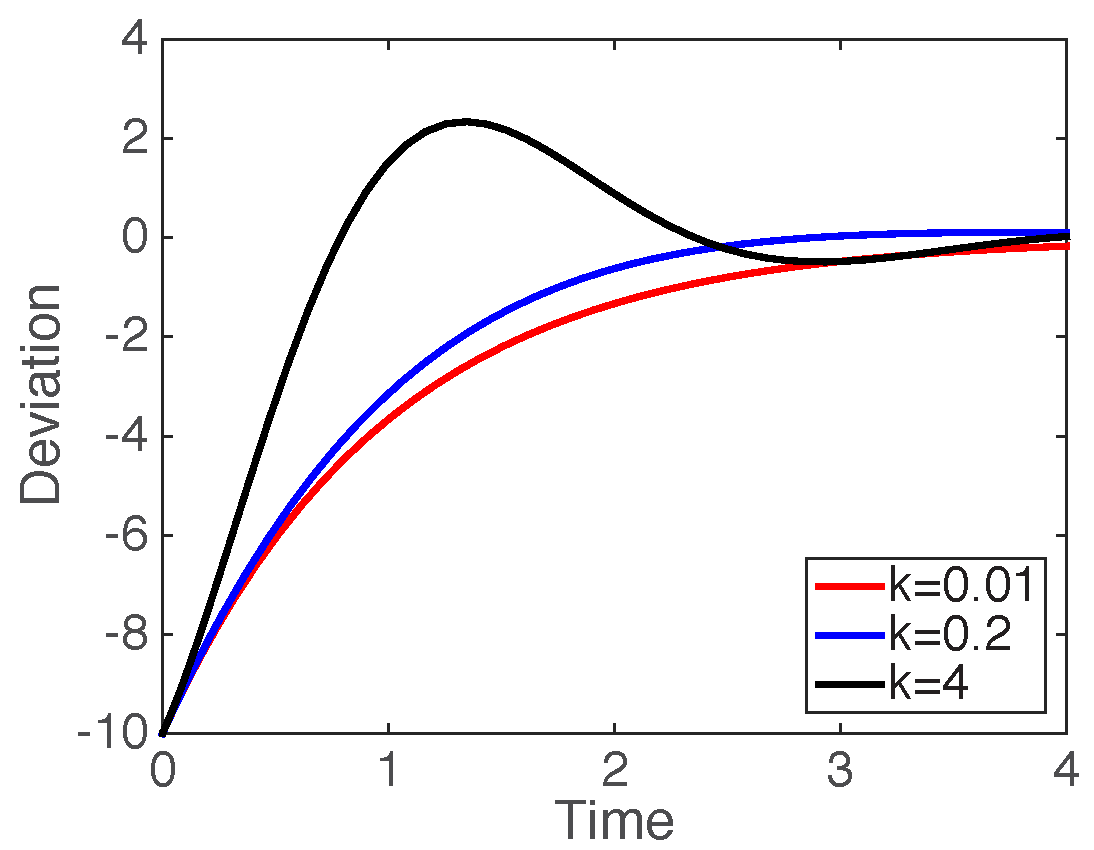
\includegraphics[width=0.4 \textwidth]{damping.pdf}\end{center}

We won't study how to identify $k^*$ in this course, but be aware of this effect.

\item Another notable shortcoming of proportional control is that it does nothing when the error term is zero. That may sound like a Yogi Berra-ism, but consider the following scenario:

\item You are driving down the highway in a car that maintains its position in a lane using proportional control. The car tracks its displacement $x$ from the midline of the lane: if $x$ is positive, it steers left, and vice versa; the angle at which it steers is proportional to the magnitude of $x$.

\item A minor quibble is that the rate at which the car approaches its desired position slows down the closer it gets, so that the car never gets exactly where it ought to be, but for the most part this strategy works fine during pleasant weather.

\item However, when a strong and persistent wind picks up, blowing the car consistently to the right. You find the car cannot ``compensate" to steer straight until it is halfway out of the lane. This is because the car will not steer far enough to the right until $x$ is fairly large.

\item In other words, even if the wind is perfectly constant, you'll be driving down the road with one tire in the shoulder. This persistent-error phenomenon is called \textit{droop} and characterizes systems with proportional control.

\item Similarly, an idealized transcriptional repressor which binds its own promoter will also have a non-zero steady-state expression level, even though negative feedback attempts to lower the repressor's concentration to zero.
\end{itemize}

\section*{Integral control}

\begin{itemize}
\item In the same constant wind, a wise driver would turn further left until reaching the middle of the lane (where the ``error" term is zero), then continue turning left just enough to compensate for the wind.

\item The driver is using memory of past errors to continue turning even when the car is on course. We call this process \textit{integral control} since it entails a response proportional to the sum of all prior errors.

\item Recall the basic Laplace transform property that $\Lapl [ \int f(t) \, dt ] = \hat{f}(s)/s$ plus a constant. Therefore a system with integral control has a feedback transfer function of the form:

\[ K(s) = \frac{1}{s \tau_i} \]

The constant $\tau_i$ is called the \textit{integral time}.

\item Integral control will eliminate the droop we saw earlier for a constant input. Recall that the error for a negative feedback loop is:


\[ \hat{y}(s) - y* = \frac{G(s) \left[ \hat{x}(s) - y^* \right]}{1 + K(s) G(s)} \]

\item As $t \to \infty$, $s \to 0$. The long-term error of the proportional control system ($K(s)=k$)  will be:

\[   \lim_{s \to 0}  \hat{y}(s) - y* = \lim_{s \to 0} \frac{G(s) \left[ \tilde{x}(s) - y^* \right]}{1 + kG(s)} \]

which is not zero in general (and particularly not when $G(s)=1/(s+a)(s+b)$, the form we saw for a biochemical cascade). However, if we have integral feedback instead so that $K(s) = 1/s\tau_i$:

\[  \hat{y}(s) - y* = \lim_{s \to 0} \frac{G(s) \left[ \tilde{x}(s) - y^* \right]}{1 + \frac{1}{s\tau_i}  G(s)} = \lim_{s \to 0} \frac{s G(s) \left[ \tilde{x}(s) - y^* \right]}{s +  \frac{1}{\tau_i}  G(s)} \]

and this limit is zero for $G(s)$ of the same form.

\item Let's compare how the two cars respond to the onset of steady gale-force winds. The proportional control car, to its credit, will begin to respond as soon as $x>0$, but will make no additional progress once its leftward steering is matched by the rightward force of the wind. The integral control car will be slower to initiate its response as the accumulated error slowly builds. However, eventually the error will be large enough that the integral control restores the correct position. At this point the integral of the error will still be positive and continue to push the car just far enough to the right to counter the wind.

\item An even better option would be to combine integral and proportional control. Then, we could combine the benefits of proportional control's faster response with integral control's long-term behavior. But is it possible to get an even faster response?

\end{itemize}
\section*{Derivative control}

\begin{itemize}
\item At the opposite end of the spectrum, there are instances when we would like a system to predict future error and provide feedback accordingly.
\item This problem is most obvious in systems when the open loop system introduces a time delay. In this case it would be helpful to know the current derivative of the error term so that we can multiply it by the time lag $\Delta t$ and add this to the current error to predict the future error -- then respond as if tha were the current error.
\item In systems that would otherwise have produced sustained oscillations, this prediction can be used to dampen the oscillations. [Plot a simple sinusoidal function and show that if the derivative $df/dt = 1$ is known when $f(t)$ = 0, the future rise in $f(t)$ can be anticipated and corrected.]
\item This type of control is called \textit{derivative control} and its feedback transfer function looks like:

\[ K(s) = s \tau_d \]

The constant $\tau_d$ is called the \textit{derivative time}.

\item Can cause wild responses to noise if not tuned properly.

\item In principle higher-order derivatives (or integrals) could be used as well, though this is not commonly done in man-made systems.
\end{itemize}

\section*{PID control}

\begin{center}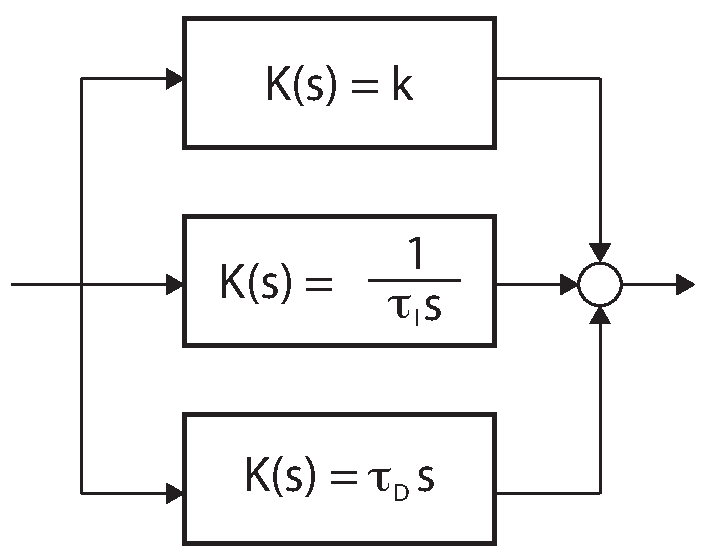
\includegraphics[width=0.5 \textwidth]{pid.pdf}\end{center}

\begin{itemize}

\item Systems that combine proportional, integral, and derivative control are used often in industry and are called PID controllers. The combined transfer function looks like:

\[ K(s) = k + \frac{\tau_i}{s} + s \tau_d   \]

\item In the next two lectures, we will see examples of integral and derivative control in biological systems as well. We'll spend the rest of today, however, discussing how we can characterize systems that use some combination of proportional, integral, and derivative control, as well as what some of their benefits are.
\end{itemize}

\section*{Transient response}

\begin{itemize}

\item The examples abovedescribe how integral and derivative control could be used to improve the longterm behavior of a system. Both types of control are also useful for transient responses (those that occur immediately after a change occurs in the input, and which die away over time).

\item Ideally we would like the transient response to die away quickly so that we reach the desired steady-state quickly. We also might prefer that the system not oscillate wildly on its way there.

\item The transient response can depend significantly on the initial conditions, but it is typical practice to assume that the initial conditions/time derivatives are all zero so that situations are comparable.

\item Questions we may ask about a system's transient response include:
\begin{itemize}
\item When does a response begin? (What is the \textit{delay time}?)
\item How long does it take for the system to traverse a specified middle range between the old and new values, e.g., from 5\% to 95\% of the new value? (What is the \textit{rise time}?)
\item How wild are the oscillations around the new steady-state value? (What is the maximum overshoot?)
\item How long until the system remains within some tolerance e.g. 5\% of the steady-state value? (What is the \textit{settling time}?)
\end{itemize}

\item It's an open question which of these qualities stand to be under the strongest selective pressure in biological systems.

\item Follow-up to in-class questions about the power of natural selection vs. drift

\begin{itemize}
\item The philosopher I mentioned, who spoke in the Department of Systems BIology two years ago, was \href{http://www.danielmilo.com/}{Daniel Milo}.
\item Milo argues that we have an exaggerated tendency to rationalize why an existing system is sensible or even ideal, \`{a} la Pangloss/Kipling. This tendency ignores the fact that a system may still be in the process of optimization, even if it has existed for a long while.
\item In particular, it may be that the fitness benefits of statistically-likely mutations are too small to permit movement towards optimality. Equivalently, we may think of a system as being trapped in a local fitness minimum from which very few and rare mutations could improve it.
\item While Milo's presentation style is deliberately provocative, the ``relative significance controversy" of drift and natural selection is a serious point of contention leading back to Fisher and Wright. (\href{http://philsci-archive.pitt.edu/1750/1/skipper_controversy.pdf}{Skipper 2002} provides a review.)
\end{itemize}


\item It may not be possible to optimize all of these qualities concurrently. For example, decreasing the rise time tends to increase the maximum overshoot. [ Reminder of the case for proportional control.]

\item The transient response will also depend on the way in which the signal changes. Depending on the relevant biological timescale, we may consider a change instantaneous (a step function) or perhaps as a ramp.

\item Fortunately, when a system has been specified, these quantities can easily be determined through algebraic manipulation and/or simulation.

\end{itemize}

\section*{Bode plots}

\begin{itemize}

\item Including all forms of control may seem the best option, but there are downsides as well that we can understand more fully by studying how each sort of control system would respond to rapid vs. slow changes.

\item A great way to do this is to study a system's response to sinusoidal inputs, $x(t)=e^{i \omega t}$. By changing the frequency $\omega$, we can adjust the speed of changes to the input

\item There is another great reason to focus on sinusoids: these are \textit{eigenfunctions} of LTI systems:

\begin{eqnarray*}
y(t) & = & h(t) \otimes x(t)\\
& = & \int_0^{\infty} h(\tau) x(t-\tau) \, d\tau\\
& = & \int_0^{\infty}h(\tau) e^{i\omega t} e^{-i\omega \tau}\, d\tau\\
& = & e^{i\omega t}  \left[  \int_0^{\infty}h(\tau) e^{-i\omega \tau}\, d\tau \right] \hspace{1 cm} \textrm{ Since } G(s) =  \int_0^{\infty}h(t) e^{-st}\, dt \\
& = & G(i\omega) e^{-\omega t}
\end{eqnarray*}

\item The output, then, is the same sinusoid multiplied by a complex number. To visualize the effect of multiplying by a complex number, let's represent $G(i\omega)$ as a complex number in argument-modulus form, $Ae^{i\phi}$:

\[ y(t) =  Ae^{i\phi} e^{i \omega t} = A e^{i \left(\omega t + \phi\right)} \]

We now recognize that the amplitude and phase of the output may differ from the input, but the frequency will stay the same.

\item If we know our system's transfer function $G(s)$, then for any given frequency $\omega$, we can calculate the amplitude and phase shift of a sinusoidal input.

\item For example, if $A \ll 1$, the system is attenuating the input -- a good thing if we are trying to buffer the output against variation in input, e.g. in a negative autoregulation system. Similarly, if $A \gg 1$, the input signal is being amplified.

\item Keeping track of the phase difference is very important in feedback loops. Imagine that we are trying to apply negative feedback to cancel out a signal $\tilde{x}(s)$ before it enters the plant. Ideally the output from the control loop is 0 degrees, 0 dB gain: that way, when we subtract it from the input, we get zero.

\item However, If the phase difference is -180 degrees, then subtracting the negative feedback is effectively the same as adding $\tilde{x}(s)$ to itself: we'd've managed to double the magnitude of the input, instead of cancelling it out!

\item Bode plots show the magnitude difference and 
address this issue by assessing the response to sinusoidal inputs with varying frequency (high freqency signals representing sudden changes and vice versa). This is achieved by plotting both the magnitude (modulus) and the phase angle (argument) of $G(i\omega)$ against $\omega$ in the manner described below.

\item Both graphs in a Bode diagram have log frequency as the independent variable. The first plots the log magnitude of $G(i\omega)$ on the y-axis: typically, we plot $20 \log_{10} | G(i \omega) |$, with units of decibels (dB).

\item This y-axis unit is not as arbitrary as it sems. The decibel unit was introduced during work on the earliest phone lines (when it was called a ``transmission unit") in order to describe the relationship between the power (``strength") of a signal at the source vs. the power at the destination.

\item The human ear perceives differences in volume on a logarithmic scale, so it was sensible to use a unit that scaled logarithmically with the ratio of the two power levels. A constant multiplier was added so that one decibel would be approximately the smallest difference in volume detectable by human ears (about a 25\% change in power):

\[ \textrm{Difference in ``volume" } = 10 \log_{10} \left( \frac{\textrm{Power at destination}}{\textrm{Power at source}} \right) \textrm{ dB} \]

\item Power is proportional to amplitude squared, so for our LTI systems the equivalent is

\[ \textrm{Signal magnitude difference: } = 20 \log_{10} \left( \frac{\textrm{Output amplitude}}{\textrm{Input amplitude}} \right) \textrm{ dB} \]

\item Follow-up to in-class question regarding why the human auditory system detects amplitude changes logarithmically:

\begin{itemize}
\item Hair cells, the primary detectors of sound, fire at a rate proportional to the logarithmic of the sound pressure (at a specific frequency). This at least rules out that the logarithmic scaling is due to downstream processing. See figure 1 of \href{http://www.ncbi.nlm.nih.gov/pmc/articles/PMC2147667/#!po=19.2308}{Dugue et al.}. However it remains unclear to me whether this is due to some property of sound transduction into the cochlea, the deflection properties of hair bundles (complicating matters each hair is coupled to the others through springs and through a membrane against which they lie, or perhaps another effect entirely.
\end{itemize}

\end{itemize}
\end{document}